\chapter[Polarization Influences the Evolution of Nucleobase -  Graphene Interactions]{Polarization Influences the Evolution of Nucleobase -  Graphene Interactions \protect\footnote[2]{This chapter has been published as \textbf{H., Hemanth} and Mallajosyula*, S.S.; Polarization Influences the Evolution of Nucleobase - Graphene Interactions; {\textit{Nanoscale}, 2021, \textbf{13}, 4060 - 4072}}}
\section{Introduction}
Graphene, a two-dimensional allotrope of carbon with hexagonal lattice has found applications in a wide range of disciplines, with electronics and material science applications at one end of the spectrum and biomedical applications at the other end.\supercite{geim_rise_2007, geim_graphene_2009, lalwani_two-dimensional_2013, akinwande_large-area_2015}  Recently, self-assembly of nucleobases on a solid support has been extensively studied in the literature, with examples of nucleobases spontaneously forming higher-order structures on metal supports like Au(111)\supercite{kelly_understanding_2008, lukas_adenine_2009} Graphene presents itself as a unique support, which can facilitate the self-assembly of nucleobases. In fact, the self-assembly of guanine nucleobases on Graphene Oxide (GO) has been studied in the literature.\supercite{chiorcea_afm_2005} The major advantage of graphene is that it can be used as an atomistically thin monolayer support to study the self-assembly of nucleobases, unlike the surface-driven assembly observed on Au(111) and Ag(111). Graphene has attracted attention as a fast and reliable tool for DNA sequencing\supercite{heerema_graphene_2016, wells_assessing_2012, dontschuk_graphene_2015, schneider_tailoring_2013} through nanopores created within the graphene sheet. Such applications are based on the non-covalent interactions present between the nucleobases and the graphene sheet, and understanding them is relevant for tuning the interactions and successfully creating nanopore based sequencing technology. Expensive QM calculations,\supercite{umadevi_quantum_2011, cho_noncovalent_2013, gowtham_physisorption_2007, umadevi_noncovalent_2014, lee_physisorption_2013} coupled with experimental studies,\supercite{varghese_binding_2009} have been employed to study the binding energies and relative orientations of the nucleobases on the graphene sheet. Multiple authors have shown that polarizability\supercite{gowtham_physisorption_2007, lee_physisorption_2013} of nucleobases play an essential role in dictating the strength of such non-covalent interactions. Computational complexities of routine QM methods such as MP2, HF and DFT which scale as O(\textit{N\textsuperscript{5}}), O(\textit{N\textsuperscript{4}}) and O(\textit{N\textsuperscript{3-4}}) respectively, limit the applicability of QM studies to smaller systems, typically one nucleobase/nucleotide interacting with a patch of the graphene sheet in a gas phase environment. This problem becomes even more challenging upon the inclusion of an explicit solvent in the calculation.

Molecular Dynamics (MD) simulations offer a viable alternative to this scenario, at the cost of high accuracy. At present, MD simulations are routinely employed to study the time evolution of large systems and help in understanding the dynamics of such systems. However, additive Force Fields (FFs) based on fixed point charges used to describe the interactions (bonded and non-bonded) in MD simulations are ill-equipped to describe the time evolution of molecular polarizability of the system. The results from MD simulations based on additive FF suggest that a subtle interplay between intermolecular hydrogen-bonding and $\pi$-$\pi$ interactions between nucleobases and the graphene sheet decides the outcome of nucleobase - graphene sheet interactions.\supercite{saikia_hierarchical_2017, saikia_dynamics_2018, ortmann_attracted_2005} However, a full-scale investigation based on the polarizable FF is absent from the literature. In this regard, we study the dynamics of nucleobases in the presence of a polarizable graphene sheet, to understand the effect of molecular polarizability on non-covalent interactions, by employing a Drude polarizable FF available in Chemistry at Harvard Molecular Mechanics (CHARMM).
\section{Computational Methodology}
Geometry optimizations for coronene were performed using the Gaussian 09 suite of programs, at the MP2/6-31G(d) level of theory. Vibration modes were also calculated at the same level of theory to ensure that the molecule was at a minimum on the potential energy surface.  Interaction energies were calculated using the ORCA suite of programs,\supercite{neese_orca_2012} at the RI-MP2/cc-pVQZ/cc-pVQZ/C level of theory from geometries optimized at the MP2/6-31G(d) level of theory. QM calculations were used to test the transfer of parameters.
\begin{figure}
    \centering
    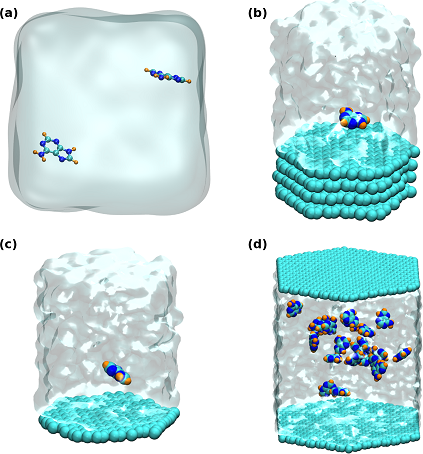
\includegraphics{Chapter1/Figures/Figure1.png}
    \caption[Representative structures for the systems considered in the present study]{Representative structures for the systems considered in the present study. (a) Free-standing nucleobases (b) Graphene - nucleobase PMF calculations using ABF simulations with multilayer graphene sheet, (c) Graphene -  nucleobase PMF calculations using ABF simulations with monolayer graphene sheet and (d) Homogeneous nucleobase- graphene system}
    \label{fig:figure17}
\end{figure}

The MD simulations were performed at the isobaric-isothermal (NPT) ensemble using the Nanoscale Molecular Dynamics (NAMD) package.\supercite{phillips_scalable_2005} CHARMM36 all-atom force field was used to describe the bonded and non-bonded interactions in graphene and nucleobases in additive FF simulations. Classical Drude polarizable FF was employed to describe the bonded and non-bonded interactions in nucleobases for Drude polarizable FF simulations. Parameters developed in-house were used to describe the bonded and non-bonded interactions in the polarizable graphene sheet. Particle Mesh Ewald (PME)\supercite{darden_particle_1993} summation was used to evaluate the electrostatic interactions with a cut-off of 9.0 $\angstrom$. Water molecules were described by the TIP3P\supercite{jorgensen_comparison_1983} water model in additive FF simulations, and the SWM4-NDP\supercite{lamoureux_polarizable_2006} polarizable water model was employed in the Drude polarizable FF simulations, with bond lengths and bond angles constrained via the SETTLE algorithm.\supercite{miyamoto_settle_1992} All simulations were performed at room temperature (298 K) with Langevin dynamics using the Nos\'{e}-Hoover Langevin piston method applied to maintain the pressure at 1 atm. For Drude FF simulations, an additional dual thermostat was employed to maintain the Drude particles in an ice bath at 1 K.

Free-standing nucleobases were modelled using CHARMM for additive FF simulations and the solvated system was simulated in a box of dimensions (30 × 30 × 30)$\angstrom$\textsuperscript{3}. We present a representative structure depicting the system setup for free-standing nucleobases in Figure 3.1(a).  Corresponding input files for the Drude polarizable FF were generated using in-house scripts. All systems were minimized with 60000 steps of CG minimization, and subsequent equilibration for 1 ns in the NPT ensemble. Production runs for additive FF simulations were run for 800 ns, while for the Drude polarizable FF simulations, production simulations were run for 2300 ns for adenine, 500 ns for guanine and thymine, and 2000 ns for cytosine. The simulations for adenine and cytosine were extended from 500 ns to 2300 ns and 2000 ns to achieve convergence.

Simulations using Adaptive Biasing Force (ABF) were also performed to estimate the binding free energies for nucleobase - nucleobase interactions and nucleobase - graphene sheet interactions. We employed a biasing force of 0.20 kcal mol\textsuperscript{-1}$\angstrom$\textsuperscript{-2} at both ends of the scan length. The scan length was divided into windows of length 0.05 $\angstrom$. We employed two methodologies to perform the ABF simulations. The first methodology was adapted from the work by Comer et al.\supercite{comer_predicting_2015,poblete_determinants_2017} In this methodology, four layers of graphene sheets were constructed to simulate a bulk graphite, with the lower sheets restrained by applying a harmonic potential. Nucleobases were placed on top of the graphene sheet and ABF simulations were performed. The ABF simulations were performed in a hexagonal unit cell of dimensions (29 x 29 x 45)  $\angstrom$\textsuperscript{3}. We present a representative structure depicting the system setup for the ABF simulations with the bulk graphite in Figure 3.1(b). In the second methodology, the ABF simulations were performed using a monolayer of graphene, to differentiate graphene and the bulk graphite. A monolayer graphene system was constructed as a hexagonal unit cell of dimensions (29 x 29 x 30) $\angstrom$\textsuperscript{3}. We present a representative structure depicting the system setup for ABF simulations with a monolayer graphene in Figure 3.1(c). Similar to the four-layer graphite system, the nucleobase was placed atop the graphene sheet. ABF scans in a nucleobase - nucleobase system were performed from 3 $\angstrom$ to 10 $\angstrom$. ABF scans in a nucleobase - graphene sheet system were performed from 3 $\angstrom$ to 15 $\angstrom$. ABF simulations for both systems were run for 100 ns in both additive and Drude FF. The simulations were deemed to have attained convergence when the number of observations in each bin was >1.5 x 10\textsuperscript{6}.

The graphene sheet was modeled using Inorganic Builder Toolkit available in VMD,\supercite{humphrey_vmd_1996} with a radius of 21 $\angstrom$ and a height of 2 $\angstrom$. We used 21 nucleobases for homogeneous nucleobase - graphene sheet simulations, and 30 nucleobases (15 of each type) in heterogeneous nucleobase - graphene sheet simulations.The graphene sheet-nucleobase system was simulated in a hexagonal unit cell of dimensions (52 × 52 × 60) $\angstrom$\textsuperscript{3}.  We present a representative structure depicting the system setup for the homogeneous nucleobase - graphene sheet simulations in Figure 3.1(d).  All systems were minimized with 60000 steps of CG minimization, and subsequent equilibration for 1 ns in the NPT ensemble. Production simulations were run for 500 ns in the NPT ensemble for additive FF, and for 500 ns in Drude FF. The equations of motion were integrated with a time step of 2 fs in additive FF simulations, while a shorter time step of 1 fs was employed in Drude polarizable FF simulations. The central atom in the graphene sheet was restrained using a harmonic potential, to ensure that the sheet does not slide during the simulations. No additional constraints were applied, and the sheets were allowed to breathe during the simulations. We note that there are a lot of reports in the literature in which the complete sheet geometry is constrained. We have ensured that the parameters allow for the ``breathing'' motion of the graphene sheets. 

Hydrogen bond and dipole moment analysis was performed using plugins available in VMD. The average number of hydrogen bonds present in the system serves as an indicator of the overall stability of the system, with a higher number of hydrogen bonds suggesting the presence of ordered structures within the system. Instances of $\pi$-$\pi$ interactions between (1) nucleobases and (2) nucleobase - graphene sheets were tracked with in-house analysis codes. Relative orientations of the nucleobases with respect to the graphene sheet were tracked to establish preferential conformations of the nucleobases in the simulation box.

\section{Results and Discussions}
\subsection{Validation of transferred parameters for the polarizable graphene sheet}
\begin{table}
	\centering
	\caption[Tansferred classical Drude Polarizable FF parameters]{Parameters transferred from benzene to graphene sheet in Drude polarizable FF. The atom descriptors are presented in Figure 3.3.}
	\begin{tabular}{cccc}
            \toprule
		Identifier	&	Parameter & Force Constant & Multiplicity\\ \midrule
		$l_{C-C}$ ($\angstrom$)	&	1.375	& 305.000&	--\\
		$l_{C-H}$ ($\angstrom$)	&	1.080	& 340.000&	--\\
        $\theta_{CCC}$(\degree)	&	120.00& 40.000& --\\
		$\theta_{CCH}$ (\degree)	&	120.00& 30.000 &--\\
		$\phi_{CCCC}$(\degree)	&	180.00  &  2.800&    2 \\
		$\phi_{CCCH}$ (\degree)	&	180.00& 4.200    &2\\
		$q_{C^\#}$	(e)&	0.0000& --&--\\
		$q_{C^\dagger}$	(e)&	0.0000& --&--\\
		$q_{C^\ddagger} $	(e)&	-0.1106& --&--\\
		$q_{H}$	(e)&	0.1106&-- &--\\
		$k_D$ (kcal/mol/$\angstrom^2$)	&	1000& --&--\\
		$\epsilon_C$ (kcal/mol)	&	-0.0690&-- &--\\
		$\sigma_C$ ($\angstrom$)	&	2.0900&-- &--  \\ \bottomrule
	\end{tabular}
 \end{table}
 
\begin{figure}
    \centering
    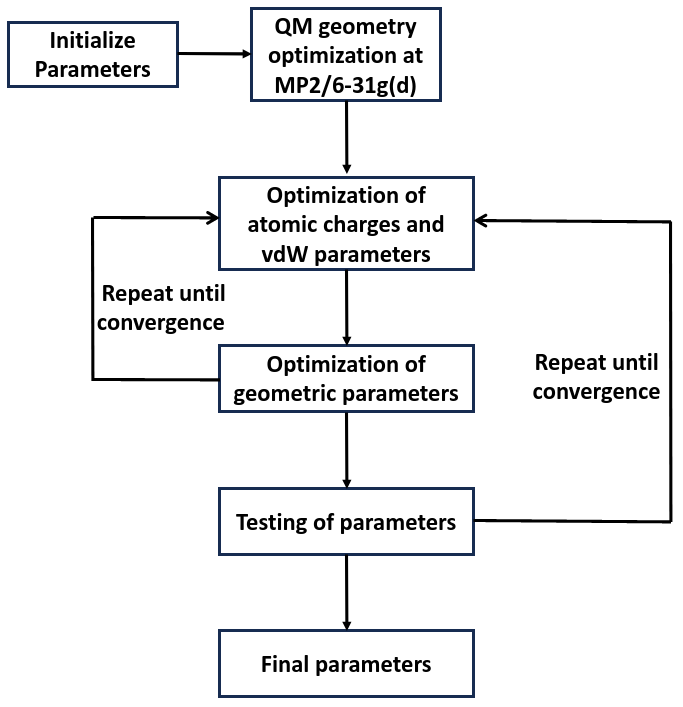
\includegraphics[width=0.6\textwidth]{Chapter1/Figures/Scheme-final.png}
    \caption[Parameterization strategy in CHARMM FF]{Parameterization strategy in CHARMM FF.}
\end{figure}

\begin{figure}
    \centering
    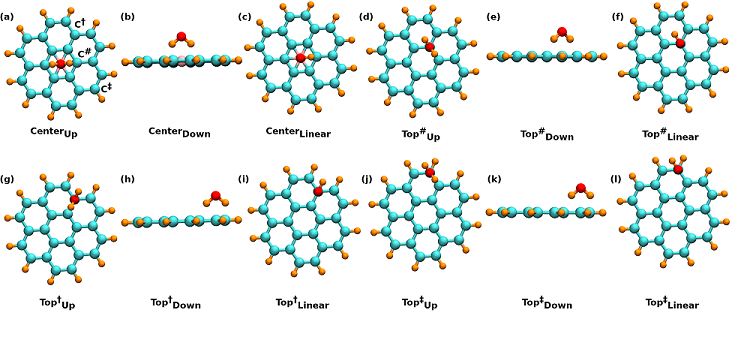
\includegraphics{Chapter1/Figures/water.png}
    \caption[Different solute-water pair interaction modes for the coronene - water model system]{Different solute-water pair interaction modes for the coronene - water model system. Carbon atoms are colored green, oxygen atoms are red and hydrogen atoms are orange. (a), (c), (d), (f), (g), (i), (j) and (l) present the top view of the concerned system, while (b), (e), (h) and (k) present the side views of the systems. C\textsuperscript{\#} forms the central six-membered ring of coronene. C$^\dagger$ corresponds to the carbon atoms on the peripheral ring, connected to the hydrogen atoms. C$^\ddagger$ corresponds to the carbon atoms on the periphery, not connected to the hydrogen atoms. All figures are generated using VMD.}
\end{figure}

The absence of suitable parameters to describe a polarizable graphene sheet necessitated the development and testing of new FF parameters to describe the graphene sheet. Towards this end, we transferred the parameters available in CHARMM Drude polarizable FF for polarizable benzene to model a polarizable graphene sheet. This transfer is analogous to the transfer of parameters from benzene to model graphene in the additive FF. The transferred parameters are presented in Table 3.1. The strategy employed for the testing of transferred parameters is presented Figure 3.2. The transferred parameters were tested using coronene as a model system for graphene, with the central six-membered ring analogous to carbons in the graphene sheet, and the external ring being analogous to the passivated ends and central pore. The transferred parameters were tested to capture the water interactions with coronene. Eight different interaction modes were considered for studying the interaction of the water molecule with the graphene sheet, which can be classified as Center, Top\textsuperscript{$\dagger$}, Top\textsuperscript{$\ddagger$} and Top\textsuperscript{\#} based on the interacting carbon atom and Up or Down based on the orientation of hydrogen atoms in the water molecule. The interaction geometries considered were based on the previous study by Schyman et al. where the adsorption of water molecules and ions was explored using OPLA-AAP FF,\supercite{schyman_exploring_2013} where it was shown that the linear approach by water molecules was disfavoured in larger carbon-based aromatic structures. All interaction modes considered are presented in Figure 3.3. The solute-water pair distances and interaction energies obtained from the QM and MM (Drude) calculations are presented in Tables 3.2 and 3.3. The interaction energies are evaluated as $E$(interaction energy) = $E$(coronene + water) - $E$(coronene) - $E$(water). These have been reported as $E$\textsubscript{QM} and $E$\textsubscript{MM}(Drude) in Table 3.3. We observed a fair reproduction of the solute-water pair interaction distances and interaction energies by the transferred parameters. The strongest interactions were observed when the water molecule approaches coronene with the hydrogens facing the sheet. The solute-water pair interaction energies calculated using RI-MP2 are also shown in Table 3.3. The parameters showed good agreement with the values obtained from QM calculations at the MP2/6-31G(d)//RI-MP2/cc-pVQZ/cc-pVQZ/C level of theory. The interaction energies and solute-water distances were also calculated at the $\omega$-B97X-D level of theory to ensure that the developed parameters are able to closely reproduce the previously reported water-interaction energy and distance reported for the system in polarizable version of the Optimized Potentials for Liquid Simulations-All Atom (OPLS-AAP) FF.

To test the applicability of the parameters developed for the polarizable graphene sheet, we calculated the binding free energies of the nucloebases to test the ability of the parameters to suitably reproduce the binding energy profiles calculated from additive and gas-phase QM simulations.

% \begin{algorithm}
%     \caption[Parameterization strategy in CHARMM FF]{Parameterization strategy in CHARMM FF.}
%     \begin{algorithmic}
%         \State Parameters $\gets$ Initialize parameters based on chemical similarity.
%         \State QM geometry $\gets$ QM geometry optimization at MP2/6-31g(d) level of theory.
%         \State QM water interaction $\gets$ QM water interactions at MP2/6-31g(d) level of theory.
%         \While{Not converged}
%             \State Optimize atomic charges and vdW parameters [Intermolecular parameters]
%             \State Optimize geometric parameters [Intramolecular parameters] 
%             \State Check convergence for both intermolecular and intramolecular parameters.
%         \EndWhile
%         \State Parameters $\gets$ Final (Optimized) FF parameters.
%     \end{algorithmic}
% \end{algorithm}

%  \begin{landscape}
    \begin{table}
        \centering
        \small
        \caption[Solute-water pair distances for the coronene - water interaction modes]{Solute-water pair distances for the coronene - water interaction modes. All distances are reported in \angstrom. MM\textsubscript{D} represents the Drude polarizable FF simulations}
            \begin{tabularx}{\textwidth}{ccccccc}
                \toprule
                Interaction                 &   MP2     &   $\omega$-B97X-D     &   MM\textsubscript{D}     &   QM\textsubscript{MP2}-MM\textsubscript{D}   &   QM\textsubscript{$\omega$-B97X-D}-MM\textsubscript{D}   &   OPLS-AAP \supercite{schyman_exploring_2013}  \\ \midrule
                Center\textsubscript{Up}    &   2.94    &   3.00    &   3.42    &   -0.48   &   -0.42   &   --  \\
                Top\textsuperscript{\#}\textsubscript{Up}   &   3.06    &   3.09    &   3.54    &   -0.48   &   -0.45   &   --  \\
                Top\textsuperscript{$\dagger$}\textsubscript{Up}    &   3.21    &   3.24    &   3.64    &   -0.43   &   -0.40       &   --  \\
                Top\textsuperscript{$\ddagger$}\textsubscript{Up}    &   3.32    &   3.29   &   3.60   &   -0.28  &   -0.31       &   --  \\ 
                Average\textsubscript{Up}   &   3.13    &   3.16    &   3.55    &   -0.42   &   -0.40   &   --  \\
                Center\textsubscript{Down}  &   3.20    &   3.27  &   3.36  &   -0.16 &   -0.09   &   3.15  \\
                Top\textsuperscript{\#}\textsubscript{Down} &   3.26    &   3.30    &   3.42    &   -0.16   &   -0.12   &   --  \\
                Top\textsuperscript{$\dagger$}\textsubscript{Down}  &   3.32    &   3.37    &   3.46    &   -0.14   &   -0.09   &   --  \\
                Top\textsuperscript{$\ddagger$}\textsubscript{Down} &   3.32    &   3.35    &   3.44    &   -0.12   &   -0.09   &   --  \\ 
                Average\textsubscript{Down}   &   3.28    &   3.32  &   3.42  &   -0.15 &   -0.10       &   3.15    \\  \bottomrule        
            \end{tabularx}
        \label{tab:my_label}
    \end{table}

    \vspace{2em}
    
    \begin{table}
        \centering
        \small
        \caption[Solute-water pair interaction energies for the coronene - water interaction modes]{Solute-water pair interaction energies for the coronene-water interaction modes. All energies are reported in kcal mol\textsuperscript{-1}. $\Delta{E}$\textsuperscript{1} = $E$\textsubscript{MM}-$E$\textsubscript{MP2}, $\Delta{E}$\textsuperscript{2} = $E$\textsubscript{MM}-$E$\textsubscript{$\omega$-B97X-D}, $\Delta{E}$\textsuperscript{3} = $E$\textsubscript{MM}-$E$\textsubscript{RI-MP2}}
            \begin{tabular}{cccccccc}
                \toprule
                Interaction                 &   $E$\textsubscript{MP2}     &    $E$\textsubscript{$\omega$-B97X-D}  &   $E$\textsubscript{RI-MP2}   &   $E$\textsubscript{MM}   &   $\Delta{E}$\textsuperscript{1}  &   $\Delta{E}$\textsuperscript{2}  &   $\Delta{E}$\textsuperscript{3}  \\ \midrule
                Center\textsubscript{Up}    &   0.15    &   -0.81   &   -1.59   &   -0.82   &   -0.97   &   -0.01   &   0.77    \\
                Top\textsuperscript{\#}\textsubscript{Up}   &   0.45  & -0.36 & -1.13 & -0.56 & -1.01 & -0.20 & 0.57 \\
                Top\textsuperscript{$\dagger$}\textsubscript{Up}   &    0.69  & 0.17  & -0.55 & -0.38 & -1.07 & -0.55 & 0.17  \\    
                Top\textsuperscript{$\ddagger$}\textsubscript{Up}   &   0.57  & 0.11  & -0.39 & -0.47 & -1.04 & -0.58 & -0.08  \\    
                Average\textsubscript{Up}   &   0.47  & -0.22 & -0.92 & -0.56 & -1.02 & -0.34 & 0.36    \\  
                Center\textsubscript{Down}    & -2.35 & -4.00 & -3.77 & -3.12 & -0.77 & 0.88  & 0.65    \\
                Top\textsuperscript{\#}\textsubscript{Down}   & -2.20 & -3.82 & -3.48 & -2.88 & -0.68 & 0.94  & 0.60 \\
                Top\textsuperscript{$\dagger$}\textsubscript{Down}   &  -1.71 & -3.15 & -2.70 & -2.32 & -0.61 & 0.83  & 0.38  \\    
                Top\textsuperscript{$\ddagger$}\textsubscript{Down}   & -1.49 & -2.92 & -2.44 & -1.91 & -0.42 & 1.01  & 0.53  \\    
                Average\textsubscript{Down}   & -1.94 & -3.47 & -3.10 & -2.56 & -0.62 & 0.92  & 0.54  \\    \bottomrule 
            \end{tabular}
        \label{tab:my_label}
    \end{table}
%  \end{landscape}

 \begin{landscape}
    \begin{table}
       \centering
       \small
       \caption[Binding free energies of nucleobases obtained from additive and Drude PMF simulations and QM calculations]{Binding free energies of nucleobases obtained from additive and Drude PMF simulations and QM calculations. All energies are reported in units of kcal mol\textsuperscript{-1}. Additive\textsuperscript{\#} and Drude\textsuperscript{\#}  correspond to PMF calculations on an unconstrained monolayer graphene sheet. Binding free energies are calculated as the difference between the energies of the equilibrium state and well-separated states. Exp. = aqueous solution and Exp.\textsuperscript{\#} = NaOH solution. Difference between the binding energies of 4-layer graphite and monolayer graphene simulations is reported in parentheses.}
       \begin{tabular}{ccccccccccc}
           \toprule
           Nucleobase  &   Additive (c36)  & Drude &   $\Delta{E}$\textsubscript{Add-Drude}    &   Additive\textsuperscript{\#} (c36)  &   Drude\textsuperscript{\#}    &  $\Delta{E}$\textsuperscript{\#}\textsubscript{Add-Drude}   &   QM  &   QM \supercite{antony_structures_2008}  &   Exp.\supercite{varghese_binding_2009}    &   Exp.\textsuperscript{\#}\supercite{varghese_binding_2009} \\ \midrule
           Adenine  & -9.40 & -8.35 & -1.05 & -8.51(-0.89) & -8.61(-0.26) & 0.10 & -17.24 & -13.6 & -6.64 & -11.85 \\
           Guanine  & -9.68 & -9.85 & 0.17  & -8.93(-0.75) & -9.51(-0.34) & 0.58 & -17.23 & -17.6 & —     & -13.45 \\
           Cytosine & -7.03 & -5.96 & -0.31 & -6.86(-0.17) & -7.87(1.91)  & 1.01 & -13.47 & -13.0 & -4.39 & -9.38  \\
           Thymine  & -7.97 & -7.66 & -1.07 & -7.73(-0.24) & -8.27(0.61)  & 0.54 & -14.33 & -14.7 & -0.68 & -4.72  \\
           Uracil   & -7.35 & -7.03 & -0.32 & -6.83(-0.52) & -7.00(-0.03) & 0.17 & -12.20 & -12.6 & —     & —     \\ \bottomrule
       \end{tabular}
       \label{tab:my_label}
    \end{table}   
   
    \begin{table}
        \centering
        \small
        \caption[Binding free energies of nucleobases obtained from additive and Drude PMF calculation for unconstrained and constrained monolayer graphene sheet]{Binding free energies of nucleobases obtained from additive and Drude PMF calculation. All energies are reported in units of kcal mol\textsuperscript{-1}. Additive\textsuperscript{\#} and Drude\textsuperscript{\#} corresponds to PMF calculations in Additive and Drude polarizable FF on an unconstrained monolayer graphene sheet. Add\textsuperscript{$\dagger$} and Drude\textsuperscript{$\dagger$} corresponds to PMF calculations calculations in Additive and Drude polarizable FF on a fully constrained monolayer graphene sheet. Binding free energies are calculated as the difference between the energies of equilibrium state and well separated states.}
        \begin{tabular}{ccccccc}
           \toprule
           Nucleobase  &   Additive\textsuperscript{\#} (c36)  &   Additive\textsuperscript{$\dagger$} (c36)   &   $\Delta{E}$\textsuperscript{\#}\textsubscript{Additive\textsuperscript{\#}-Additive\textsuperscript{$\dagger$}} &   Drude\textsuperscript{\#}   &   Drude\textsuperscript{$\dagger$}    &   $\Delta{E}$\textsuperscript{\#}\textsubscript{Drude\textsuperscript{\#}-Drude\textsuperscript{$\dagger$}}     \\ \midrule
           Adenine  & -8.51 & -9.06 & 0.55 & -8.35 & -8.92 & 0.57  \\
           Guanine  & -8.93 & -9.41 & 0.48 & -9.85 & -9.76 & -0.09 \\
           Cytosine & -6.86 & -6.89 & 0.03 & -5.96 & -6.64 & 0.68  \\
           Thymine  & -7.73 & -8.47 & 0.74 & -7.66 & -6.32 & -1.34 \\
           Uracil   & -6.83 & -7.03 & 0.20 & -7.03 & -6.86 & -0.17 \\ \bottomrule
        \end{tabular}
        \label{tab:my_label}
    \end{table}
 \end{landscape}

 \subsection{Potential of mean force calculations}
 \begin{figure}
    \centering
    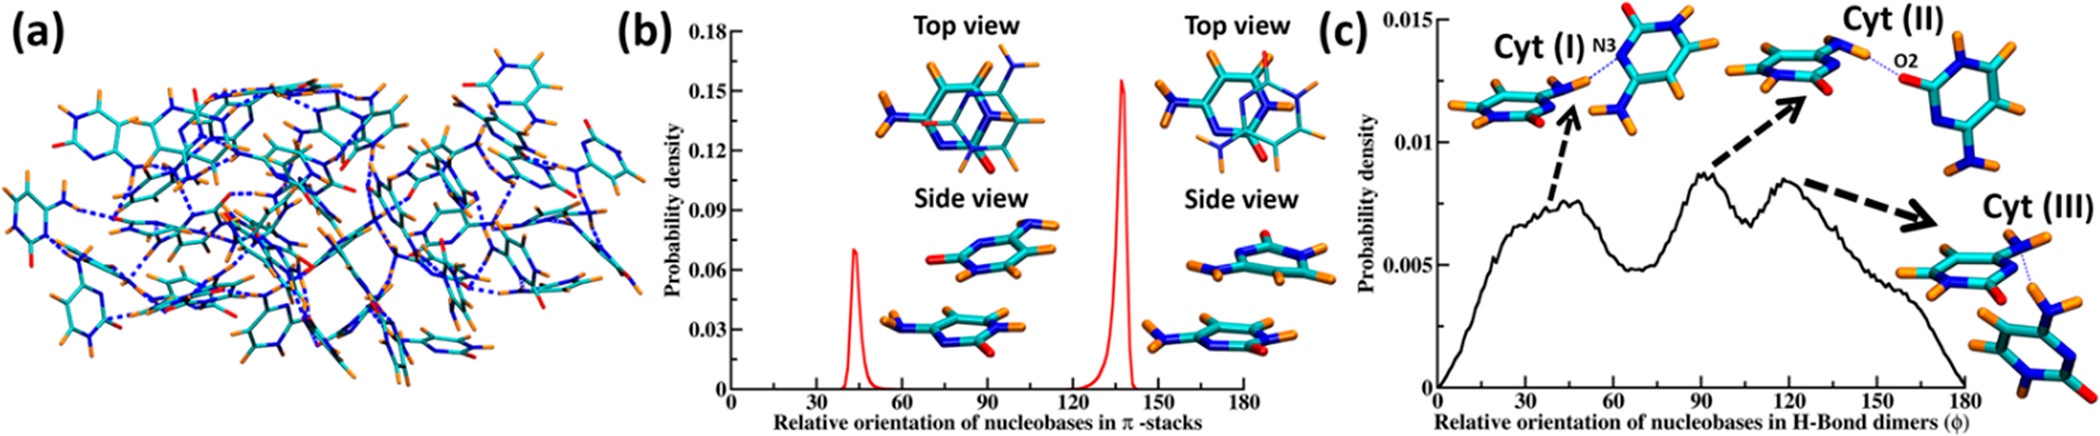
\includegraphics{chapter1/Figures/Figure3.png}
    \caption[Representative image for scan coordinate in nucleobase - graphene sheet ABF simulations]{Representative image for scan coordinate in nucleobase - graphene sheet ABF simulations.}
 \end{figure}
 \begin{figure}
    \centering
    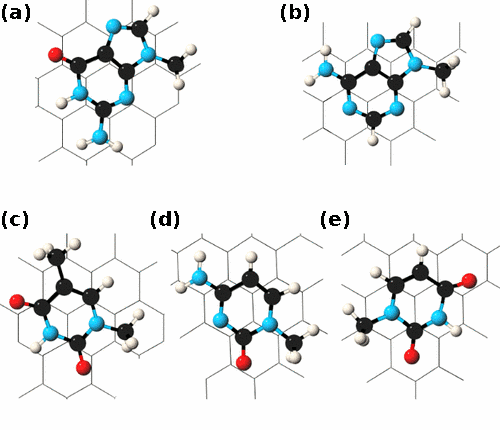
\includegraphics{chapter1/Figures/Figure2.png}
    \caption[Potential of Mean Force (PMF) of the five nucleobases: adenine, thymine, guanine, cytosine and uracil, respectively]{Potential of Mean Force (PMF) of the five nucleobases: adenine, thymine, guanine, cytosine and uracil, respectively.}
 \end{figure}
 Potential of Mean Force (PMF) was calculated for the adsorption of the nucleobases (adenine, guanine, thymine, cytosine and uracil) on the graphene sheet to estimate the effect of polarization on the binding free energies. The scan coordinate used for evaluating the nucleobase - graphene sheet PMF is presented in Figure 3.4.  PMF scans obtained from additive, Drude polarizable FF and QM calculations are presented in Figure 3.5. Binding free energies estimated from additive and Drude simulations of the four-layer graphite and monolayer graphene are presented in Table 3.4. The binding free energies from the Drude (additive) simulations from the four-layer graphite ABF simulations for the five nucleobases G, A, T, C and U were found to be -9.85 (-9.68), -8.35 (-9.40), -7.66 (-7.97), -5.96 (-7.03) and -7.03 (-7.35), respectively. The binding free energies from the Drude (additive) simulations from the monolayer graphene ABF simulations for the five nucleobases G, A, T, C and U were found to be -9.51 (-8.93), -8.61 (-8.51), -8.27 (-7.73), -7.87 (-6.86) and -7.00 (-6.83), respectively. All energies are presented in kcal mol\textsuperscript{-1}. We find that the inclusion of polarizability makes it easier to adsorb and desorb nucleobases from the bulk graphite. The binding free energies for A and C are -1.05 kcal mol\textsuperscript{-1} and -1.07 kcal mol\textsuperscript{-1} lower respectively in classical Drude polarizable FF simulations, when compared to the additive simulations for the bulk graphite system. The influence of polarization on G, C and U was minimal when compared to A and T for the bulk graphite system. In terms of the absolute values, the binding free energies follow the trend G > A > T > U > C in both Drude and additive simulations of the bulk graphite systems. For the monolayer systems, the binding energies of C, G and T are 1.01 kcal mol\textsuperscript{-1}, 0.58 kcal mol\textsuperscript{-1} and 0.54 kcal mol\textsuperscript{-1} higher respectively in classical Drude polarizable FF simulations, when compared to the additive simulations. The influence of polarization on A and U was minimal when compared to that on G, C and T for the monolayer graphene system. We find that the inclusion of polarizability makes it harder to adsorb and desorb nucleobases from the monolayer graphene. In terms of the absolute values, the binding free energies follow the trend G > A > T > C > U in both Drude and additive simulations of the monolayer graphene systems. We note that while the inclusion of polarization makes it easier to desorb nucleobases from graphite, the same favours strong adsorption over the monolayer graphene. However, in both the cases, the maximum change is of the order of 1 kcal mol\textsuperscript{-1}. This is in agreement with the experimental observations by Varghese et al.\supercite{varghese_binding_2009}, and theoretical calcultaions by Grimme et al.\supercite{antony_structures_2008} The graphene-nucleobase interaction energies calculated using isothermal titration calorimetry in aqueous (alkaline) solution reported by Varghese et al. for G, A, T and C were found to be nil (-13.45), -6.64 (-11.85), -0.68 (-4.72) and -4.34 (-9.38), respectively (interaction energies could not be calculated for guanine in aqueous solution due to the insolubility of guanine in aqueous solution).  All energies are reported in kcal mol\textsuperscript{-1}. We observe that the values obtained using both the Drude and additive simulations lie between the experimental values obtained for aqueous and alkaline solutions. Additionally, we also performed ABF simulations with a constrained graphene sheet to probe the influence of structural fluctuations in the graphene monolayer on the adsorption of the nucleobases. The binding free energies are tabulated in Table 3.5. For the additive simulations, we observe that the average difference in the binding free energies upon constraining the sheet is 0.4 kcal mol\textsuperscript{-1}. The maximum difference was observed for T with the binding free energy being 0.74 kcal mol\textsuperscript{-1} higher upon constraining the sheet. For Drude simulations, the maximum difference in binding free energies between an unconstrained and constrained sheet was observed for T and C. For T, we observe that constraining the sheet lowered the binding free energy with the difference being -1.34 kcal mol\textsuperscript{-1}, while for C constraining the sheet increases the binding energy with the difference being 0.68 kcal mol\textsuperscript{-1}. From both additive and Drude simulations, we note that constraining the sheet influences the binding energetics and must be accounted for in the simulations.
 
 \subsection{Nucleobase - nucleobase interactions}
 Before studying the interaction of the nucleobases with the graphene sheet, we also estimated the influence of polarization on the nucleobase - nucleobase interactions. We estimated the binding free energies of nucleobase - nucleobase interactions by studying the dynamics of a two nucleobase system via an unbiased simulation and an adaptive biasing force (ABF) simulation. The unbiased simulations were run for 800 ns and 500 ns for the additive and Drude FF, respectively. The simulations for adenine and cytosine were extended to 2300 ns and 2000 ns, respectively, to ensure convergence. In the ABF simulations, the scan coordinate was defined as the distance between the center of mass (COM) of the two nucleobases. In Figure 3.6, we present a representative illustration of the scan coordinate. In Figures A.1 and A.2 of the Appendix A, we present the time series corresponding to the distance between the COM of the two nucleobases and the relative orientation between the two nucleobases for the additive and Drude simulations, respectively. The PMF plots obtained for the nucleobase-nucleobase interactions from the additive and Drude simulations are presented in Figure A.3 in the Appendix A. The structures corresponding to the minima observed from the PMF calculations for nucleobase-nucleobase interactions are presented in Figure 3.7.

    \begin{figure}
        \centering
        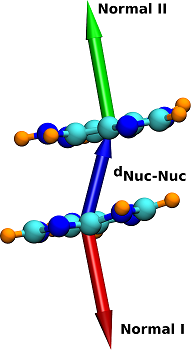
\includegraphics{Chapter1/Figures/Figure4.png}
        \caption[Representative image for scan coordinate in nucleobase - nucleobase ABF simulations]{Representative image for scan coordinate in nucleobase - nucleobase ABF simulations. Orientation of nucleobases are  calculated from the normal vectors of molecular planes, as \textit{arccos(NormalI · NormalII)}.}
    \end{figure}

    \begin{table}
        \centering
        \caption[Binding free energies of nucleobase - nucleobase interactions obtained from additive and Drude simulations]{Binding free energies of nucleobase - nucleobase interactions obtained from additive and Drude simulations. All energies are reported in units of kcal mol\textsuperscript{-1}. Binding free energies are calculated as the difference between the energies of the equilibrium state and the well-separated states. Binding energies from the unbiased simulations are reported in parentheses. dA, dC, dT and U correspond to deoxyadenosine, deoxythymidine, deoxycytidine and uridine, respectively.}
        \begin{tabular}{ccccc}
            \toprule
            Nucleobase & additive & Drude\textsubscript{$\pi$-stacking} & Drude\textsubscript{Hbond} & Expt.\supercite{schyman_exploring_2013} \\ \midrule
            Adenine & -1.54(-1.23) & -2.17(-1.20) & -1.50(dA)	& -5.62(-5.02) \\
            Guanine & -1.74(-1.36) & -1.96(-1.75) & - & -1.95(-1.21) \\
            Cytosine & -0.42(-0.09) & 0.66(0.34) & 0.06(dC) & -2.03(-2.59) \\
            Thymine & -0.99(-0.72) & 0.95(-0.29) & 0.06(dT) & -0.57(-0.23) \\
            Uracil & -0.54(-0.69) & -0.61(-0.45) & 0.21(U) & -0.39(-0.21) \\ \bottomrule
        \end{tabular}
    \end{table}

    \begin{figure}
        \centering
        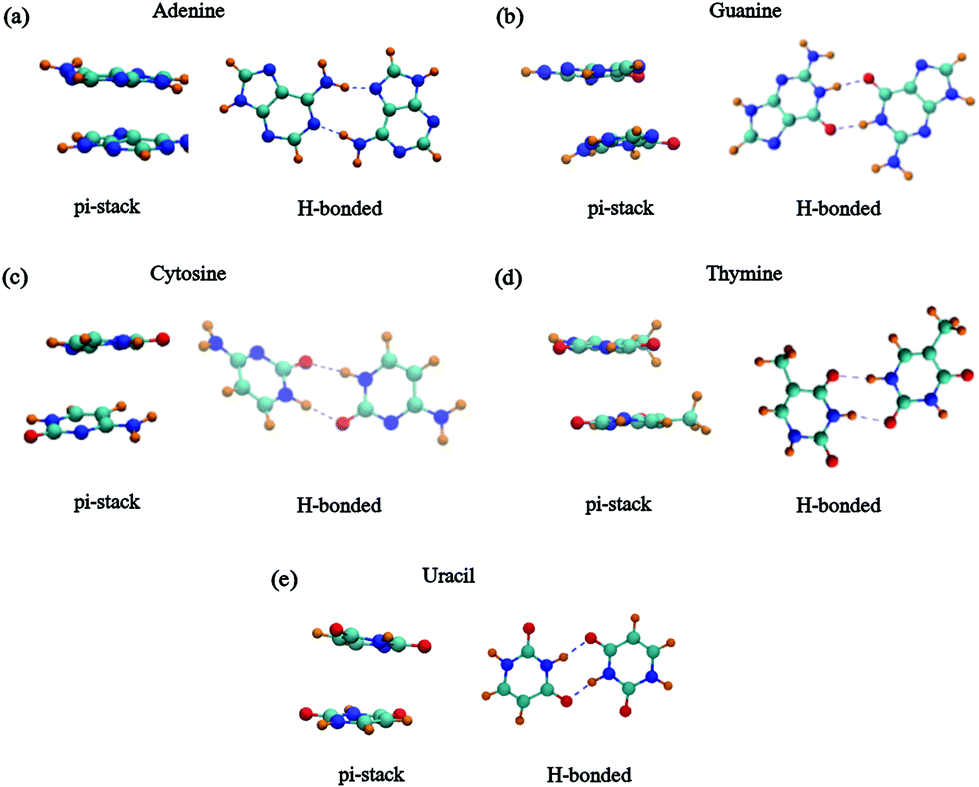
\includegraphics[width=\textwidth]{Chapter1/Figures/Figure6.png}
        \caption[Representative structures corresponding to various minima observed in the PMF curves for Adenine, Guanine, Cytosine, Thymine and Uracil nucleobases.]{Representative structures corresponding to various minima observed in the PMF curves for (a) Adenine, (b) Guanine, (c) Cytosine, (d) Thymine and (e) Uracil nucleobases.}
    \end{figure}

    We observe that adenine forms an unsymmetrical hydrogen-bonded dimer, while other nucleobases favour the formation of symmetrical dimers. It was also observed that all nucleobases were preferentially adopting a slip-stacked arrangement in $\pi$-stacked configurations. We observed a satisfactory overlap between the binding energies obtained from both the unbiased and ABF simulations in both additive and Drude simulations. On comparing the additive and Drude simulations, we also observe distinct signatures of the influence of polarization.  Additive simulations predominantly favor only the $\pi$-stacking conformations for all the nucleobases, while in the Drude simulations, we observe both hydrogen bonding and $\pi$-stacking conformations.  In fact, hydrogen bonding was observed to be the preferred mode of interaction for all the nucleobases, except guanine, where both $\pi$-stacking and hydrogen bonding were equally favoured. Binding free energies for $\pi$-stacking obtained from additive and Drude simulations are presented in Table 3.6. For the additive simulations, we observe that both the ABF and unbiased simulations predict the binding free energy trend as G > A > T > U > C, with the binding free energy values ranging between -1.74 (-1.36) kcal mol\textsuperscript{-1} and -0.42 (-0.09) kcal mol\textsuperscript{-1} from the ABF (unbiased) simulations. From the Drude simulations, we observe that the unbiased simulations predict the trend, G > A > U > T > C, with the free energy values ranging between -1.75 kcal mol\textsuperscript{-1} and 0.34 kcal mol\textsuperscript{-1}. However, the ABF simulations predict the trend to be A > G > U > C > T with the free energy values ranging between -2.17 kcal mol\textsuperscript{-1} and 0.95 kcal mol\textsuperscript{-1}. Experimental studies by Solie and Schellman using thermal osmometry have earlier reported that the interactions between nucleobases and nucleosides in aqueous solution are mediated via $\pi$-stacking of nucleobases.\supercite{solie_interaction_1968} Stacking free energies from their experimental studies for deoxyadenosine, deoxythymidine, deoxycytidine and uridine were found to be -1.50 kcal mol\textsuperscript{-1}, 0.06 kcal mol\textsuperscript{-1}, 0.06 kcal mol\textsuperscript{-1} and 0.21 kcal mol\textsuperscript{-1}, respectively. The same have been reported in Table 3.6.  We observe that the values obtained from both Drude and additive simulations are in agreement with the experimental values. We note that the experimental studies were performed on nucleosides, while our results are for nucleobases. Binding free energies corresponding to the formation of hydrogen-bonded dimers observed in Drude simulations are also presented in Table 3.6. Both the ABF and unbiased simulations show that adenine favors the formation of hydrogen bonds (-5.62 and -5.02 kcal mol\textsuperscript{-1}), followed by cytosine (-2.03 and -2.59 kcal mol\textsuperscript{-1}) and guanine (-1.95 and 1.21 kcal mol\textsuperscript{-1}), while thymine (-0.57 and -0.23 kcal mol\textsuperscript{-1}) and uracil (-0.39 and -0.21 kcal mol\textsuperscript{-1}) do not favor the formation of hydrogen-bonded dimers. The formation of adenine and guanine tetrads via intermolecular hydrogen-bonding is well known in the literature.\supercite{verma_many_2010, burge_quadruplex_2006, cassidy_guanine-centric_2014} The formation of hydrogen-bonded stabilized adenine dimers in solution has also been observed by infrared spectroscopy.\supercite{hamlin_hydrogen-bonded_1965}

    Based on the satisfactory reproduction of nucleobase - graphene sheet binding energies and an insight into the energetics of the nucleobase - nucleobase interactions, we study the self-assembly of nucleobases on a graphene sheet. We follow the dynamics of a homogeneous nucleobase - graphene system for five nucleobases, and also consider a heterogeneous (GC/AT) base pair - graphene system. Each system was simulated for 500 ns using the additive FF and for 500 ns using the Drude FF.
    \subsection{MD Simulations}
    \subsubsection{Homogeneous nucleobase - graphene system}
    We study the evolution of the interactions between the nucleobases and the underlying graphene sheet by performing a time-series analysis for two collective variables: (i) distance between the COM of the nucleobase and the graphene sheet (d\textsubscript{Nuc-Graph}) and (ii) relative orientations of the nucleobase with respect to the graphene sheet ($\theta$\textsubscript{Nuc-Graph}). In Figure 3.8 we illustrate both the collective variables. The time series corresponding to the additive and Drude simulations are presented in Figures A.4 and A.5 of the Appendix A. The convergence of the simulations was addressed using the time series analysis. For the additive simulations, we observed that the nucleobases, irrespective of their chemical identity, preferentially interacted with the graphene sheet to form a monolayered assembly. All the nucleobases were observed to drift towards the graphene sheet and form a stable monolayer within the first 100 ns. The last 350 ns of the additive simulations were used for further analysis. Similarly in Drude simulations, we found that all the nucleobases, except guanine, interacted preferentially with the graphene sheet forming a stable mono-layer. Guanine was found to form multiple layers stabilized by $\pi$-$\pi$ interactions between guanine nucleobases. We observe that fluctuations in the COM time series cease beyond 150 ns. The last 350 ns of the Drude simulation trajectories were used for further analyses presented in the paper. 
    \begin{figure}
        \centering
        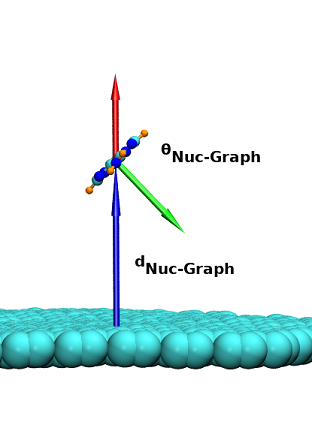
\includegraphics{Chapter1/Figures/cv.png}
        \caption[Representative illustration of the CVs used to study the evolution of the interactions between the nucleobases and the underlying graphene sheet]{Representative illustration of the CVs used to study the evolution of the interactions between the nucleobases and the underlying graphene sheet. Relative orientations are calculated as \textit{arccos(z-axis * Normal)}. d\textsubscript{Nuc-Graph} is evaluated as the difference between z-coordinates of COM of nucleobase and graphene sheet.}
    \end{figure}

    In Figure 3.9(a) we present the distribution corresponding to the distance between the COM of the nucleobase and the graphene sheet (d\textsubscript{Nuc-Graph}). We clearly observe the formation of a monolayer for all nucleobases expect guanine, highlighting the fact that nucleobases tend to interact preferentially with the graphene sheet. The average d\textsubscript{Nuc-Graph} distances for adenine, cytosine, thymine and uracil were found to be 3.44 (3.62) $\angstrom$, 3.56 (3.62) $\angstrom$, 3.56 (3.73) $\angstrom$ and 3.92 (4.61), respectively, in additive (Drude) simulations. For guanine, in the Drude simulations, the bases arranged themselves to form 5 distinct layers at distances 3.66 $\angstrom$, 6.77 $\angstrom$, 10.09 $\angstrom$, 13.45 $\angstrom$ and 16.78 $\angstrom$ from the graphene sheet, as shown in Figure 3.9(b). The average d\textsubscript{Nuc-Graph} distance for guanine from the additive simulation was 3.67 $\angstrom$. In Figure A.5 of the Appendix A, we we also present the distribution of the relative orientations of the nucleobase with respect to the graphene sheet. We observe that all the nucleobases lie flat on the graphene sheet or within the stacks formed in the guanine Drude simulations.
    \begin{figure}
        \centering
        \includegraphics[width=\textwidth]{Chapter1/Figures/FigureCOM.png}
        \caption[Distribution of d\textsubscript{Nuc-Graph} of nucleobases: adenine, guanine, cytosine, thymine and uracil, respectively. Snapshot from the simulation trajectory of guanine showing the $\pi$-stack formation]{ (a) Distribution of d\textsubscript{Nuc-Graph} of nucleobases: adenine, guanine, cytosine, thymine and uracil, respectively. Signatures of $\pi$-stacks formed by guanine nucleobases in Drude simulations are discernible from the plot. (b) Snapshot from the simulation trajectory of guanine showing the $\pi$-stack formation.}
    \end{figure}

    The results observed by us for the additive simulations are in agreement with the earlier reports by Saikia et al.,\supercite{saikia_hierarchical_2017, saikia_dynamics_2018} wherein cytosine and guanine were found to preferentially tile the surface of the graphene sheet. Thus, we note that for the additive simulations, the nucleobase - nucleobase interactions die out quickly, as the nucleobase - graphene sheet $\pi$-interactions become dominant. However, in the Drude simulations, we observe the formation of $\pi$-stacks and even hydrogen-bonded structures.
    \begin{figure}
        \centering
        \includegraphics[width=\textwidth]{Chapter1/Figures/dipole_new.png}
        \caption[Probability distribution of instantaneous dipole moments for the nucleobases: adenine, guanine, cytosine, thymine and uracil, respectively]{Probability distribution of instantaneous dipole moments for the nucleobases: adenine, guanine, cytosine, thymine and uracil, respectively. Dipole moments are reported in units of Debye.}
    \end{figure}
    
    In an attempt to understand the influence of molecular polarizability on non-covalent interactions, we analyzed the instantaneous dipole moments of the nucleobases over the length of the simulation trajectory from both the nucleobase only and nucleobase - graphene simulations. The probability distributions of the instantaneous dipole moments from both the additive and Drude FF simulations are presented in Figure 3.10. We observe that the dipole moments from the Drude simulations are shifted to larger values when compared to the additive simulations. The average dipole moments from the nucleobase - graphene additive (Drude) simulations for A, G, C, T and U were found to be 3.0 (4.0) D, 7.6 (9.4) D, 8.2 (12.1) D, 4.6 (7.9) D and 4.5 (6.3) D, respectively. We found that the distribution of dipole moments did not show a strong dependency on the formation of self-assembled structures in the simulations. It was observed that the distributions of instantaneous dipole moments obtained from freebase and nucleobase - graphene sheet simulations showed an appreciable overlap in both additive and Drude simulations. This was especially true for the purine nucleobases, where no influence of the graphene sheet was observed on the values of the instantaneous dipole moments. For the pyrimidine nucleobases, we find a slight shift in the average dipole moment value in the presence of the graphene sheet. For cytosine, the value increased from 11.9 D to 12.1 D, while for T the value decreased from 8.3 D to 7.8 D. We note that this may be due to the formation of strong hydrogen-bonding observed in thymine.

    Finally, we analyze the simulations for the formation of local hydrogen-bonded structures on the graphene sheet. Nucleobases are known to form hydrogen-bonded self-assemblies on two dimensional supports such as Au(111) and Ag(111).\supercite{ciesielski_self-assembly_2016} Formation of the hydrogen-bonded ordered structures for nucleobases on the graphite surface has been observed for adenine,\supercite{freund_structure_1997} guanine\supercite{heckl_two-dimensional_1991} and uracil.\supercite{sowerby_scanning_1997} The experimental studies using scanning tunnelling microscopy (STM) and low-energy electron diffraction (LEED) found that the nucleobases formed a close-packed network of hydrogen-bonded dimers. Stability of the hydrogen-bond stabilized dimer and higher ordered structures were evaluated as a function of the probability of occurrence. We employed a cut-off of >25\% occurrences to classify the hydrogen-bonded structures as significant. We did observe the formation of hydrogen-bonded structures in additive simulations; however, the probabilities of these dimeric structures were found to be <25\%.  We note that this observation is in accordance with the earlier reports by Saikia et al.,\supercite{saikia_hierarchical_2017,saikia_dynamics_2018} who observed a dispersive behaviour for guanine and cytosine on graphene surfaces at low concentrations. For Drude simulations, we observed the formation of hydrogen-bonded structures even at the low concentrations (0.25 M) studied by us. The structures were found to be predominantly dimeric in nature, with the probabilities of the formation of stable dimeric structures for adenine, guanine, cytosine, thymine and uracil being between 33.45\%-50.76\%, 28.67\%-75.21\%, 33.92\%-88.20\%, 29.24\%-69.29\% and 39.20\%-75.06\%, respectively. In Figure A.6 of Appendix A, we present the probability of the formation of dimer pairs as a heat map. We observed the formation of 15, 15, 21, 9 and 4 dimers in adenine, guanine, cytosine, thymine and uracil simulations, respectively. To ascertain the lifetime for the dimer pairs, we also evaluated the hydrogen bond auto-correlation function. The plots for the hydrogen bond auto-correlation function are presented in Figure 3.11. The average lifetimes of the dimer pairs obtained by fitting the auto-correlation function using a two-term exponent are tabulated in Table 3.7 for both the additive and Drude polarizable FF simulations. The average lifetimes are found to be 23.68 ps and 65.11 ps for the additive and Drude simulations, respectively.
    \begin{figure}
        \centering
        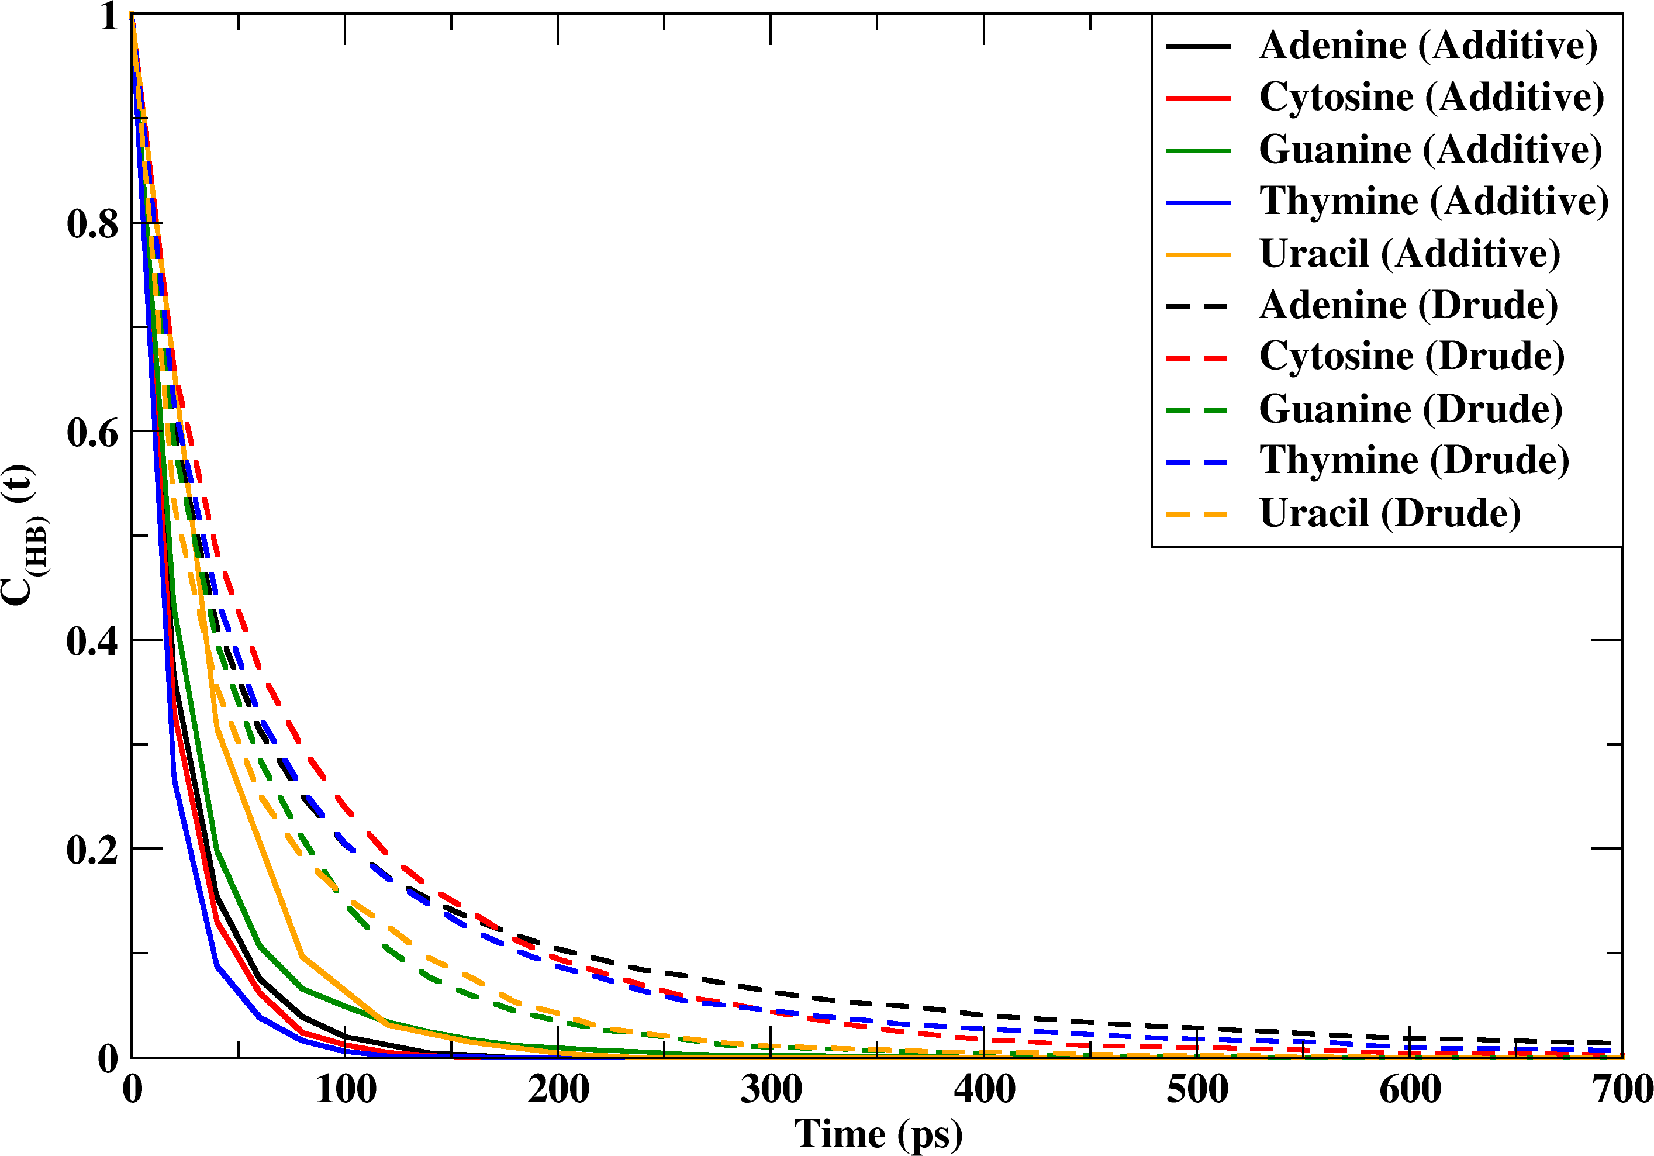
\includegraphics[width=\textwidth]{Chapter1/Figures/autocorrelation.png}
        \caption[Comparison of continuous hydrogen-bond auto-correlation function for the dimer pairs in the simulation systems]{Comparison of continuous hydrogen-bond auto-correlation function for the dimer pairs in the simulation systems.}
    \end{figure}
    \begin{table}
        \centering
        \caption[Average lifetimes of the hydrogen bonded dimers observed in the nucleobases for additive and Drude polarizable FF simulations.]{Average lifetimes of the hydrogen bonded dimers observed in the nucleobases for additive and Drude polarizable FF simulations. Lifetimes are calculated by fitting to a two term-exponential}
        \begin{tabular}{ccc}
            \toprule
            Nucleobase  &   $\tau$\textsubscript{additive}(ps)  &   $\tau$\textsubscript{Drude}(ps) \\ \midrule
            Adenine     &   21.73   &   79.86   \\
            Guanine     &   28.08   &   49.73   \\
            Cytosine    &   19.39   &   74.94   \\
            Thymine     &   14.49   &   71.88   \\
            Uracil      &   34.72   &   49.17   \\
            $\tau$\textsubscript{Average}   &   23.68   &   65.11   \\ \bottomrule
        \end{tabular}
    \end{table}
    \begin{figure}
        \centering
        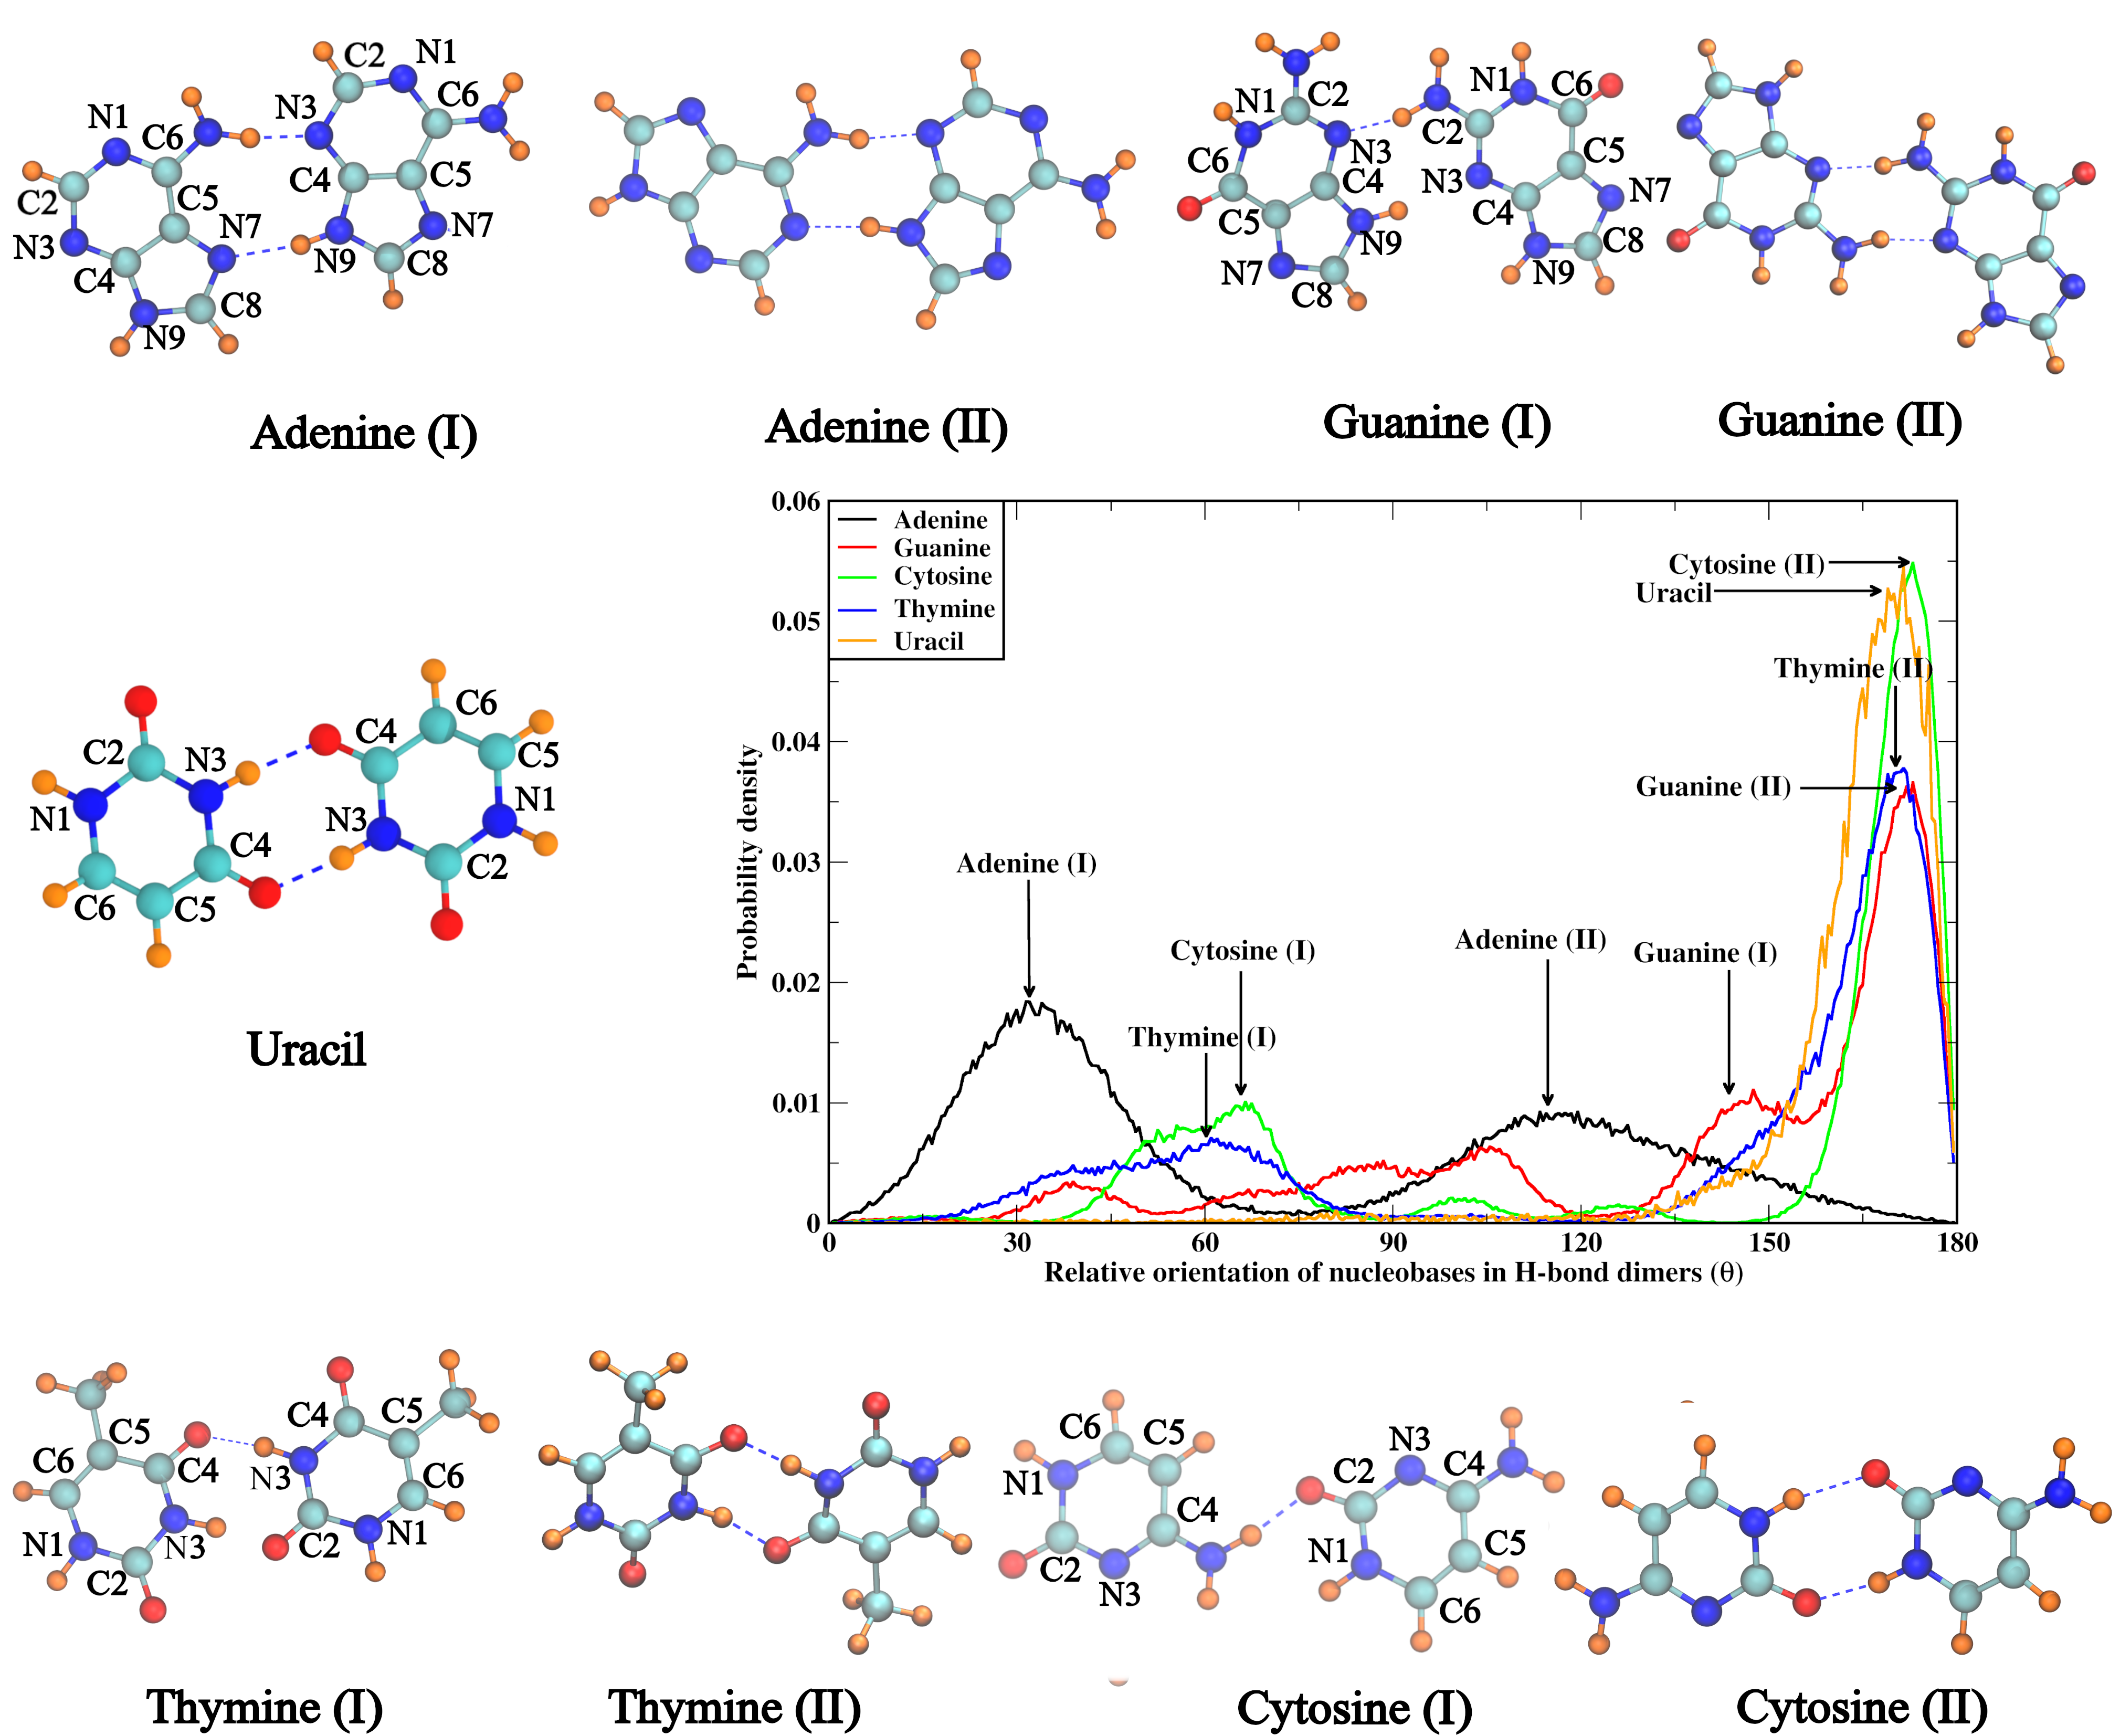
\includegraphics[width=\textwidth]{Chapter1/Figures/hbonds_full_mod_new1.png}
        \caption[Relative orientation of nucleobases in hydrogen-bonded dimers observed in homogeneous Drude FF simulations. Structures corresponding to the most significant hydrogen-bonded dimer pairs have also been presented]{Relative orientation of nucleobases in hydrogen-bonded dimers observed in homogeneous Drude FF simulations. Structures corresponding to the most significant hydrogen-bonded dimer pairs have also been presented. Carbon atoms are coloured green, nitrogen atoms are blue, oxygen atoms are red and hydrogen atoms are orange.}
    \end{figure}
    % \begin{figure}
    %     \centering
    %     \includegraphics[width=\textwidth]{Chapter1/Figures/adenine_network_compressed.png}
    %     \caption[ Representative image showing various hydrogen-bonded structures formed by Adenine on graphene sheet]{ Representative image showing various hydrogen-bonded structures formed by Adenine on graphene sheet}
    % \end{figure}
    \begin{table}
        \centering
        \caption[Prominent Hbonds between nucleobases in homogeneous nucleobase - graphene Drude polarizable FF simulations]{Hbond pairing among the nucleobases in homogeneous nucleobase - graphene Drude polarizable FF simulations.}
        \begin{tabular}{cccc}
            \toprule
            Structure   & Nucleobase 1  & Nucleobase 2  & Orientation (\degree)\\ \midrule
            Adenine(I)  & -NH$_2$       & N3            & 31.5\degree \\
                        & N7            & N9 \\ 
            Adenine(II) & -NH$_2$       & N3            & 113.5\degree \\
                        & N1            & N9 \\ 
            Guanine(I)  & -NH$_2$       & N3            & 145\degree \\
            Guanine(II) & -NH$_2$       & N3            & 173\degree \\ 
                        & N3            & -NH$_2$ \\ 
            Cytosine(I) & -NH$_2$       & C2(O)         & 67\degree \\ 
            Cytosine(II)& C2(O)         & N1            &   173\degree\\ 
                        & N1            & C2(O) \\ 
            Thymine(I)  &   C4(O)       &   N3          &   60\degree   \\
            Thymine(II) &   C4(O)       &   N3          &   173\degree  \\
                        &   N3          &   C4(O)   \\  
            Uracil      &   C4(O)       &   N3          &   173\degree  \\
                        &   N3          &   C4(O)   \\      \bottomrule
        \end{tabular}
    \end{table}

    \begin{figure}
        \centering
        \includegraphics{Chapter1/Figures/cytosine_figure1.png}
        \caption[Representative image showing the self-organised C1-D(2) ribbon-type higher-order structures formed by cytosine on the graphene sheet.]{Representative image showing the self-organised C1-D(2) ribbon-type higher-order structures formed by cytosine on the graphene sheet.}
    \end{figure}
    
    Upon analyzing the structural characteristics of the dimer pairs, we observed that the various dimeric assemblies formed amongst the nucleobases could be classified using the relative orientation of the bases in the dimer pairs. Hydrogen-Bonded dimer pairs were identified by enforcing a distance cut-off of 3.0 $\angstrom$ between the hydrogen-bond donor (D) and acceptor (A) atoms, and an angle cut-off of 20$\degree$ between the vectors lying along D-H and H-A bonds. In Figure 3.12, we present the relative orientation of the nucleobases in hydrogen-bonded dimer pairs. For adenine, we find the formation of two unique dimer pairs with a relative average orientation of 31.5$\degree$ [adenine(I)] and 113.5$\degree$ [adenine(II)]. The conformations corresponding to adenine(I) and adenine(II) are presented in Figure 3.12.  In both adenine(I) and adenine(II), we observe the formation of two hydrogen-bonds between the adenine nucleobases. The atoms involved in the formation of the hydrogen-bonds are listed in Table 3.8.  Besenbacher et al. used ab initio calculations to explore the various dimeric structures, which could be formed in adenine and cytosine monolayers deposited on the Au(111) surface.\supercite{kelly_understanding_2008, lukas_adenine_2009} The dimeric structures formed within the simulation cell for adenine, adenine(I) and adenine(II) are consistent with the structures A\textsubscript{1}A\textsubscript{5} and A\textsubscript{2}\={A}\textsubscript{5} reported by Besenbacher et al.\supercite{kelly_understanding_2008} using ab initio calculations and STM observations. In Figure A.7 of the Appendix A, we present representative snapshots of the self-assembly of adenine dimers on the graphene sheet. For guanine, cytosine and thymine, we find the formation of a dominant hydrogen-bonded dimer with a relative angle of 173$\degree$ when compared to adenine, wherein we observed two hydrogen-bonded dimers with similar occurrences.  In Figure 3.12, we also present the conformations corresponding to these dominant hydrogen-bonded dimers for guanine, cytosine and thymine. In contrast to the adenine hydrogen-bonded dimers for guanine, cytosine, thymine and uracil, we observe the formation of symmetric hydrogen-bonded dimers, with the same atoms being involved in the formation of hydrogen-bonds in the two nucleobases. For guanine(II), the hydrogen-bonds are formed between the amino (-NH\textsubscript{2}) group and the N3 nitrogen, for cytosine(II) the hydrogen-bonds are formed between the C2 carbonyl oxygen and the N1 nitrogen, for thymine(II) the hydrogen-bonds are formed between the C4 carbonyl oxygen and the N3 nitrogen, and for uracil the hydrogen-bonds are formed between the C4 carbonyl oxygen and the N3 nitrogen. The other hydrogen-bonded structures among guanine, cytosine and thymine (guanine(I), cytosine(I) and thymine(I)) were found for transient structures with only one hydrogen-bond between the nucleobases. It is interesting to note that the symmetric dimers found in guanine, cytosine, thymine and uracil have been observed in experimental assemblies.\supercite{kelly_understanding_2008, lukas_adenine_2009, sowerby_scanning_1997, otero_elementary_2008, spada_guanosine-based_2008, xu_probing_2007} The guanine dimer with hydrogen-bonds between the amino (-NH\textsubscript{2}) group and the N3 nitrogen has been observed to be an integral part of the G-ribbon B structure reported by Spada et al.,\supercite{spada_guanosine-based_2008} wherein the guanine nucleobases were self-assembled on a graphite support. The cytosine dimer structure, with hydrogen-bonds between the C2 carbonyl oxygen and the N1 nitrogen, has been observed to be a part of the C-1D(2) ribbon structure studied by Besenbacher et al.\supercite{otero_elementary_2008} for the cytosine assemblies on the Au(111) support. It was found that cytosine could assemble into multiple patterns on the Au(111) support by the formation of zigzag filaments and five- and six-membered rings. Central to all these self-assemblies was the formation of various dimeric conformations between the cytosine nucleobases, highlighting the importance of dimerization in the self-assembly.  In Figure 3.13, we present a snapshot from the Drude simulations, wherein we observed the self-assembly of the cytosine dimers to aggregate and form C-1D(2) ribbon-like structures observed by Besenbacher et al.\supercite{otero_elementary_2008} for the cytosine assemblies on the Au(111) support. Similar to the pattern formation in cytosine, Besenbacher et al. also studied the formation of supramolecular assemblies in thymine.\supercite{xu_probing_2007} The thymine dimers reported by us were observed in the island structures of thymine assemblies on the Au(111) support. Uracil dimers reported by us were observed in the herringbone structures of uracil assemblies on graphite and molybdenum disulphide surfaces.\supercite{sowerby_scanning_1997,sowerby_molecular_1998}

    \subsubsection{Heterogeneous nucleobase - graphene system}
    Nucleobases have the unique ability to form specific inter-molecular hydrogen-bonds, which leads to the formation of well-known Watson-Crick base pairs between adenine : thymine and guanine : cytosine. To explore the formation of such base pairs, we analyze two sets of heterogeneous systems, adenine with thymine and guanine with cytosine, to explore the spontaneous formation of hydrogen-bond stabilized base pairs over the graphene sheet. The simulation cell consisted of 15 nucleobases of purine (A/G) and pyrimidine (T/C) type, accounting for 30 nucleobases per cell. Heterogeneous simulations were performed at a concentration of 0.16 M. We restrict the analyses to only Drude polarizable FF simulations, wherein we observed significant aggregation and higher-order structures.
    \begin{figure}
        \centering
        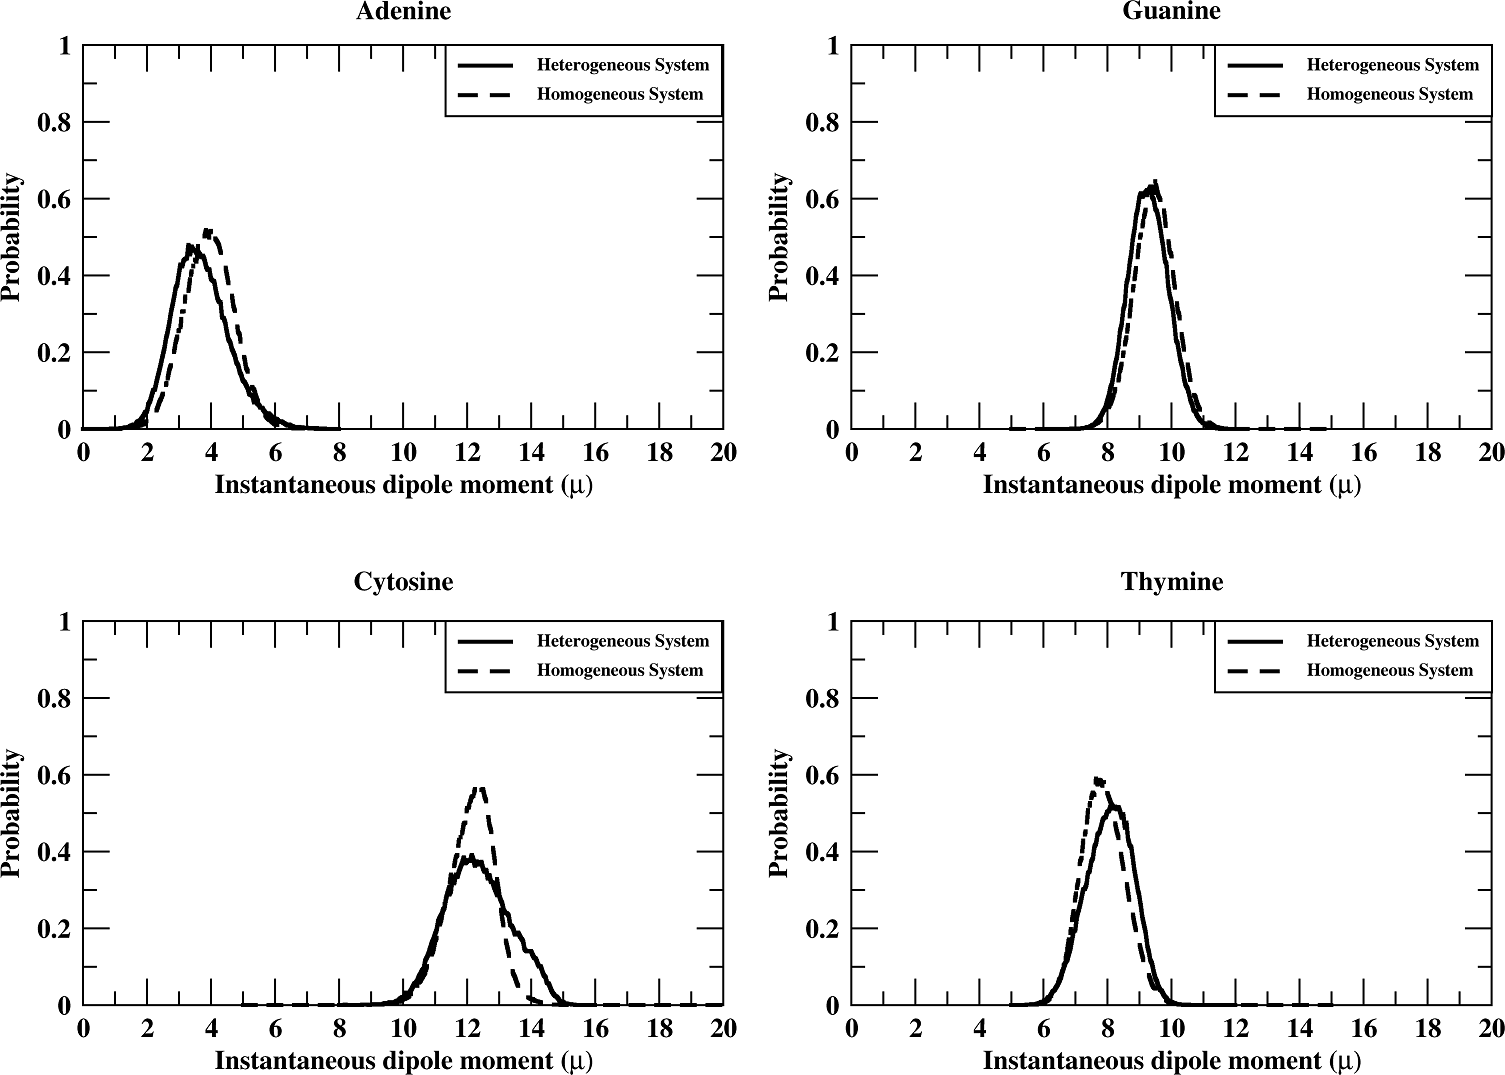
\includegraphics[width=\textwidth]{Chapter1/Figures/hetdipole.png}
        \caption[Probability distribution of Instantaneous dipole moments for nucleoobases; Adenine, Guanine, Cytosine, Thymine and Uracil respectively]{Probability distribution of Instantaneous dipole moments for nucleoobases; Adenine, Guanine, Cytosine, Thymine and Uracil respectively. Dipole moments are reported in units of Debye}
    \end{figure}
    We analysed the instantaneous dipole moments over the length of the trajectory for heterogeneous nucleobase - graphene simulations, and the results were compared with the values obtained from the homogeneous nucleobase - graphene simulations. The probability distributions of instantaneous dipole moments from both homogeneous and heterogeneous nucleobase - graphene simulations are presented in Figure 3.14. The average dipole moments from homogeneous and heterogeneous nucleobase - graphene simulations of the DNA nucleobases are presented in Table 3.9. The average dipole moments from the heterogeneous nucleobase - graphene (homogeneous) simulations for A, G, C and T were found to be 3.7 (4.0) D, 9.3 (9.4) D, 12.3 (12.1) D and 8.0 (7.9) D, respectively. The difference in dipole moments is also presented in Table 3.9. We observed that the dipole moments from heterogeneous simulations undergo shifts when compared to the homogeneous simulations. Dipole moments of purine nucleobases: adenine ($\Delta\mu$ = -0.3) and guanine ( $\Delta\mu$ = -0.1) were found to shift to lower values in comparison with the values from the homogeneous simulations. The dipole moments of cytosine ( $\Delta\mu$ = 0.2) and thymine ( $\Delta\mu$ = 0.1), being pyrimidine nucleobases, underwent shifts towards higher values in comparison with the homogeneous simulations. We note that our results are in line with the observations in base flipping.\supercite{lemkul_induced_2014} However, the magnitude of change in dipole moment is less compared to base flipping.
    \begin{table}
        \centering
        \caption[Instantaneous dipole moments of nucleobases from homogeneous and heterogeneous nucleobase - graphene simulations]{Instantaneous dipole moments of nucleobases from homogeneous and heterogeneous nucleobase - graphene simulations}
        \begin{tabular}{cccc}
            \toprule
            Nucleobase  &   Dipole moment ($\mu$)   &   Dipole moment ($\mu$)   & $\Delta\mu$\\
                        &   homogeneous             &   heterogeneous           &           \\  \midrule
            Adenine     &   4.0                     &   3.7                     &   -0.3    \\
            Guanine     &   9.4                     &   9.3                     &   -0.1    \\
            Cytosine    &   12.1                    &   12.3                    &   0.2     \\
            Thymine     &   7.9                     &   8.0                     &   0.1     \\  \bottomrule
        \end{tabular}
    \end{table}
    
    We next investigate the formation of hydrogen-bonded structures in the heterogeneous systems. Using the same distance and angle cut-offs to identify a hydrogen bond as discussed for the homogeneous system, we identify hydrogen-bonded dimer pairs in the heterogeneous system. We did not observe significant formation of hydrogen-bonded structures from the heterogeneous nucleobase - graphene sheet simulations using additive FF. We have presented the heat maps depicting the probabilities of the formation of various dimer pairs from the additive FF simulations in Figure A.8 of the Appendix A. For the Drude simulations we observed that in the heterogeneous system, the hydrogen bonds are only observed between purine and pyrimidine bases, i.e. between adenine and thymine or guanine and cytosine. We did not observe hydrogen bonds between purine bases or pyrimidine bases such as A : A, T : T, G : G or C : C. The probabilities of the formation of dimeric structures were between 52.62\%-83.71\% and 39.14\%-90.16\% for the adenine - thymine and guanine - cytosine pairs, respectively. We observed the formation of 10 dimers in the adenine - thymine and guanine - cytosine simulations, respectively. The probabilities of the formation of various heterogeneous nucleobase dimer pairs from the Drude polarizable FF simulations are presented as a heat map in Figure A.9 in Appendix A.
    \begin{figure}
        \centering
        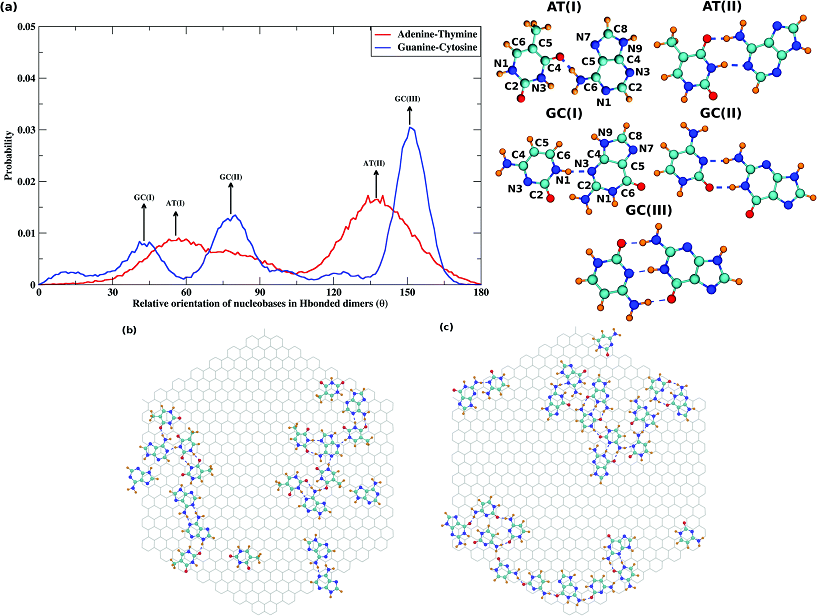
\includegraphics[width=\textwidth]{Chapter1/Figures/Figurelast.png}
        \caption[Relative orientation of nucleobases in the hydrogen-bonded dimers observed in heterogeneous Drude FF simulations. Structures corresponding to the most significant hydrogen-bonded dimer pairs have also been presented]{(a) Relative orientation of nucleobases in the hydrogen-bonded dimers observed in heterogeneous Drude FF simulations. Structures corresponding to the most significant hydrogen-bonded dimer pairs have also been presented. Carbon atoms are coloured green, nitrogen atoms are blue, oxygen atoms are red and hydrogen atoms are orange. Representative image showing higher-order structures in (b) A : T and (c) G : C simulations.}
    \end{figure}

    In Figure 3.15(a), we present the relative orientation of the nucleobases involved in hydrogen-bonded dimers. We use this analysis to identify the distinct interaction modes between the nucleobases. For adenine and thymine dimer pairs, we observe a bimodal distribution for the relative orientations centered at 31.5$\degree$ [AT(I)] and at 113.5$\degree$ [AT(II)]. The first peak [AT(I)] corresponds to the formation of a single hydrogen bond between A and T, which is also reflected by the broad distribution. The second peak (AT(II)) corresponds to the formation of the conventional Watson-Crick hydrogen-bonded structure, with two hydrogen bonds between A and T. The representative structures of the hydrogen-bonded dimers and the atoms involved in the hydrogen-bonds are presented in Fig. 3.14(a). The atoms involved in the formation of hydrogen-bonds are listed in Table 3.10. For guanine and cytosine dimer pairs, we observe three distinct peaks in the distribution for the relative orientations centered at 41$\degree$ [GC(I)], 80$\degree$ [GC(II)] and 151$\degree$ [GC(III)], respectively. The representative structures corresponding to these peaks are presented in Figure 3.15(a). We observe that these distributions correspond to the formation of a single hydrogen-bond [GC(I)], two hydrogen-bonds [GC(II)] and three hydrogen-bonds[GC(III)] between guanine and cytosine. GC(III) corresponds to the canonical Watson-Crick hydrogen-bonded structure. The atoms involved in the hydrogen-bonds are presented in Table 3.10.
    \begin{table}
        \centering
        \caption[hydrogen-bond pairing among the nucleobases in the heterogeneous nucleobase - graphene simulation]{hydrogen-bond pairing among the nucleobases in the heterogeneous nucleobase - graphene simulation}
        \begin{tabular}{cccc}
            \toprule
            Structure   &   Nucleobase I            &   Nucleobase II           &   Orientation     \\   \midrule
            AT(I)       &   -NH\textsubscript{2}    &   N3                      &   31.5$\degree$   \\
                        &   N7                      &   N9                                          \\
            AT(II)      &   -NH\textsubscript{2}    &   N3                      &   113.5$\degree$  \\
                        &   N1                      &   N9                                          \\  
            GC(I)       &   N1                      &   N3                      &   41$\degree$     \\
            GC(II)      &   N3                      &   -NH\textsubscript{2}    &   80$\degree$     \\
                        &   C2(O)                   &   N1                                          \\
            GC(III)     &   C2(O)                   &   -NH\textsubscript{2}    &   115$\degree$    \\
                        &   N3                      &   N1                                          \\
                        &   -NH\textsubscript{2}    &   C6(O)                                       \\  \bottomrule
        \end{tabular}
    \end{table}

    We also analysed if the dimeric structures aggregated within the simulation cell to form higher-order assemblies. The ability of the nucleobases to form single and multiple hydrogen-bonds in A : T and G : C pairs enables the formation of higher-ordered structures, instead of dimers dispersed over the graphene sheet. Using STM imaging, Besenbacher et al. observed the formation of ordered structures for A : T and G : C pairs co-adsorbed on the HOPG surface.\supercite{mamdouh_supramolecular_2006,xu_coadsorption_2006} From the heat maps presented in Figure A.9 of the Appendix A, we observe the occurrences of a nucleobase being hydrogen-bonded to more than one partner. In Figures 3.15(b) and (c), we present representative snapshots of higher-order structures observed by us in A : T and G : C simulations. We observe that the structures are stabilized by different combinations of hydrogen-bonds, and are in agreement with the experimental results.

    \section{Conclusions}
    In summary, the results from the present study show a qualitative and quantitative agreement with the previously reported results in the literature, while improving upon the parameters available in the literature to describe a polarizable graphene sheet. We show that the inclusion of polarizability affects the outcome of simulations for both free-standing nucleobases and nucleobase - graphene sheet systems. It is shown that polarizability plays a crucial role in determining the fate of non-covalent interactions within the simulation cell. The observance of $\pi$-$\pi$ stacking interactions in guanine is consistent with the experimental observation of a strong hydrophobic-driven assembly in guanine nucleobases\supercite{varghese_binding_2009} and poly-G single strands,\supercite{akca_competing_2011} an effect which is not captured by additive simulations. The polarizable simulations were also able to accurately capture the observed phenomenon of the formation of H-bond stabilized dimers,\supercite{kelly_understanding_2008,lukas_adenine_2009,otero_elementary_2008,spada_guanosine-based_2008,xu_probing_2007} in contrast to additive simulations where no H-bond formation was observed amongst the nucleobases. We were also able to study the spontaneous formation of ordered self-assemblies in adenine and cytosine nucleobase-graphene systems, which have not been observed in additive simulations. We also explored the formation and dynamics of ordered self-assemblies in heterogeneous nucleobase - graphene sheet simulations. The study sheds light on the relative strengths of nucleobase - graphene sheet interactions and nucleobase - nucleobase interactions, and how the subtle interplay between the various forces dictates the evolution of the system. The parameters for the polarizable graphene sheet would also enable the study of other interfacial phenomena at the graphene surface.